\documentclass[8pt,a4paper,notitlepage]{scrartcl}
\usepackage[left=0.5cm, right=0.5cm, top=0.5cm, bottom=0.5cm]{geometry}
\usepackage[utf8]{inputenc} % for direct umlaut input
\usepackage[T1]{fontenc}    % for umlaut encoding
\usepackage[english]{babel}
\usepackage[pdfusetitle]{hyperref}
\usepackage{fancyhdr}
\renewcommand{\headrulewidth}{0pt}
\pagestyle{fancy}
\fancyhf{}
\usepackage{amssymb,amsmath,graphicx,xcolor,url,qrcode,bm,physics,booktabs,dsfont,slashed,multicol}
\usepackage{verbatim}
\usepackage[most]{tcolorbox}
\renewcommand{\familydefault}{\sfdefault}
\parskip = 10pt plus 30pt minus 8pt
% NEW COMMANDS %%%%%%%%%%%%%%%%%%%%%%%%
\colorlet{boxBG}{black!3!white}
\colorlet{boxFrame}{black!12!white}
\colorlet{boxTitle}{black!85!white}
\colorlet{mainFont}{black!85!white}
\colorlet{codeFont}{red!85!black}
\newcommand{\im}[0]{\mathrm{i}}
\newcommand{\eu}[0]{\mathrm{e}}
\renewcommand{\vec}[1]{\bm{#1}}
\renewcommand{\Tr}[1]{\operatorname{Tr}\left\{#1\right\}}
\newcommand{\id}[0]{\mathds 1}
\newcommand{\codebox}[2]{\begin{tcolorbox}[
  colback=boxBG,
  colframe=boxFrame,
  coltitle=mainFont,
  coltext=mainFont,
  left=1pt,
  right=1pt,
  top=1pt,
  bottom=1pt,
  bottomtitle=0mm,
  toptitle=0mm,
  title=\textbf{#1},
  halign title=left, 
  after={\par}]
#2
\end{tcolorbox}}
\newcommand{\mycode}[2]{#1: \\\color{codeFont}\texttt{> #2}\color{mainFont}}
\newcommand{\mylineLong}[0]{\color{boxFrame}\hspace{-1.6mm}\rule[0.6mm]{98mm}{.5mm}\color{mainFont}}
\newcommand{\mylineShort}[0]{\color{boxFrame}\rule[0.6mm]{60.5mm}{.4mm}\color{mainFont}}
\newcommand{\newitem}[0]{\\[3pt]}
% BEGIN DOCUMENT %%%%%%%%%%%%%%%%%%%%
\begin{document}
\color{mainFont}

\begin{multicols}{3}
[
{\noindent\LARGE \textbf{\href{https://matplotlib.org/}{Matplotlib v3.4.2} Cheat Sheet}} \qquad\texttt{import numpy as np; import matplotlib.pyplot as plt; plt.style.use('science')}
]

\codebox{Preparing the Data}{
\color{codeFont}
\texttt{> t = np.linspace(0, 2*np.pi, 500) \\
> x, y = np.sin(t), np.cos(t) \\
> data1 = [10, 20, 40, 80] \\
> data2 = [12, 18, 48, 66] \\
> labels = ['A', 'B', 'C', 'D'] \\
> data3 = np.random.randn(300) \\
> data4 = np.random.randn(300) * 2 \\
> X, Y = np.meshgrid(t, t) \\
> Z = (np.sin(X) + np.cos(Y))**2
}
\color{mainFont}
}

\codebox{Single 2D Line Plot}{
\color{codeFont}
\texttt{> fig, ax = plt.subplots(figsize=(5,3)) \\
> ax.set\_xlim(t[0], t[-1]) \\
> ax.set\_ylim(-1.2, 1.2) \\
> ax.set\_xlabel(r'time') \\
> ax.set\_ylabel(r'position') \\
> ax.plot(t, x, c='r', label=r'one') \\
> ax.fill\_between(t, x, y, alpha=0.1, \\
. \ \ \ \ \ \ \ \ \ \ \ \ \ \ \ color='g') \\
> ax.plot(t, y, c='b', label=r'two') \\
> ax.legend(title='Title') \\
> ax.set\_title(r'Oscillation of \$f(x)\$') \\
> ax.annotate(r'\$\textbackslash swarrow\$', (3.4,0)) \\
> plt.savefig('figure.pdf')
}
\color{mainFont}
\begin{center}
	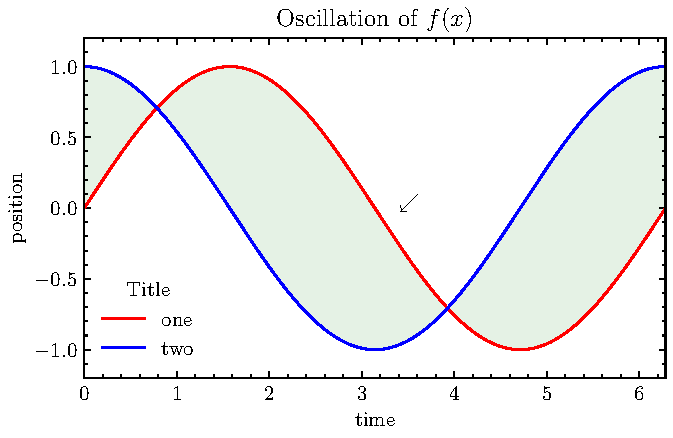
\includegraphics[width=0.9\textwidth]{fig-single.pdf}
\end{center}
}

\codebox{Multiple 2D Plots}{
\color{codeFont}
\texttt{> fig, axes = plt.subplots(2, 1, \\
. \ \ \ \ \ \ \ \ \ \ \ \ \ \ \ \ \ \ \ \ \ \ \ \ figsize=(5,3)) \\
> ax = axes[0] \\
> ax.plot(t, x, t, y, linestyle=":") \\
> ax = axes[1] \\
> ax.plot(t, x+y, t, x-y)
}
\color{mainFont}
\begin{center}
	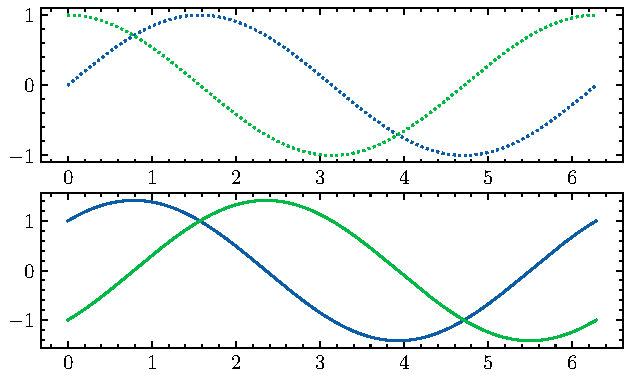
\includegraphics[width=0.9\textwidth]{fig-multi.pdf}
\end{center}
}

\codebox{Logarithmic Plots}{
\color{codeFont}
\texttt{> fig, ax = plt.subplots(figsize=(5,2)) \\
> ax.set\_xscale('log') \\
> ax.plot(t, x, t, y)
}
\color{mainFont}
\begin{center}
	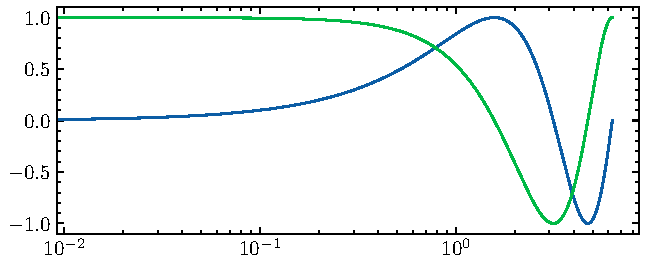
\includegraphics[width=0.9\textwidth]{fig-logscale.pdf}
\end{center}
}

\codebox{Line Styles}{
\begin{center}
	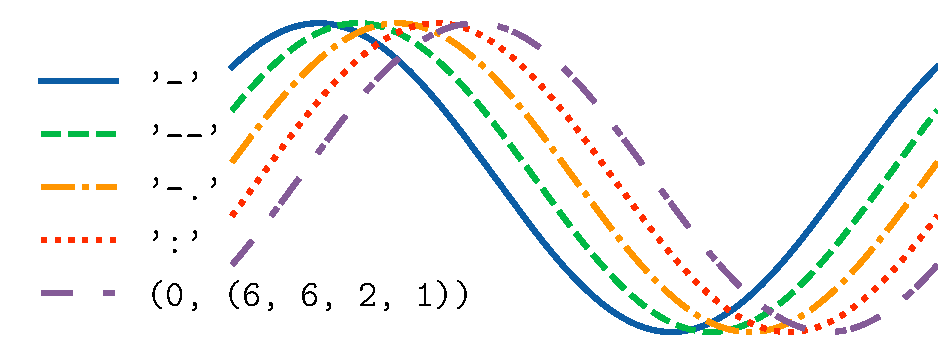
\includegraphics[width=\textwidth]{fig-plot-markers.pdf}
\end{center}\vspace{-0.15cm}
\texttt{(0, (6, 6, 2, 1))}: 0pt offset, 6pt line, 6pt space, 2pt line, 1pt space, and then repeat. 
}

\codebox{Scatter Plot}{
\color{codeFont}
\texttt{> fig, ax = plt.subplots(figsize=(5,3)) \\
> ax.scatter(data3, data4, marker='.')\vspace{-0.4cm}
}
\color{mainFont}
\begin{center}
	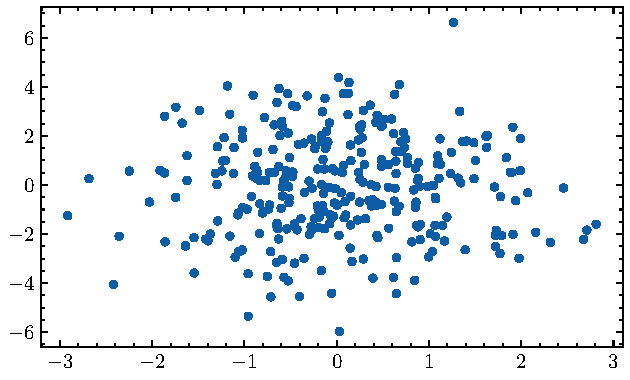
\includegraphics[width=0.9\textwidth]{fig-scatter.pdf}
\end{center}
}

\codebox{Scatter Markers}{
\begin{center}
	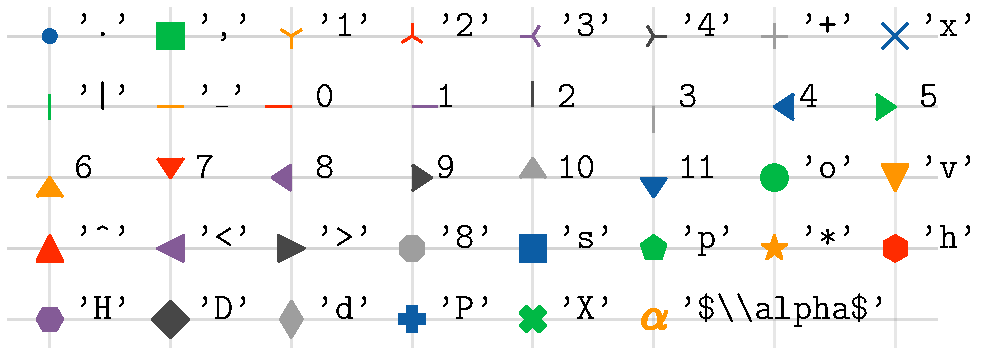
\includegraphics[width=\textwidth]{fig-scatter-markers.pdf}
\end{center}
}

\codebox{Bar Chart}{
\color{codeFont}
\texttt{> l, w = np.arange(len(labels)), 0.35 \\
> fig, ax = plt.subplots(figsize=(5,3)) \\
> ax.bar(l - w/2, data1, w, label='a') \\
> ax.bar(l + w/2, data2, w, label='b') \\
> ax.set\_xticks(l) \\
> ax.set\_xticklabels(labels) \\
> ax.legend()\vspace{-0.15cm}
}
\color{mainFont}
\begin{center}
	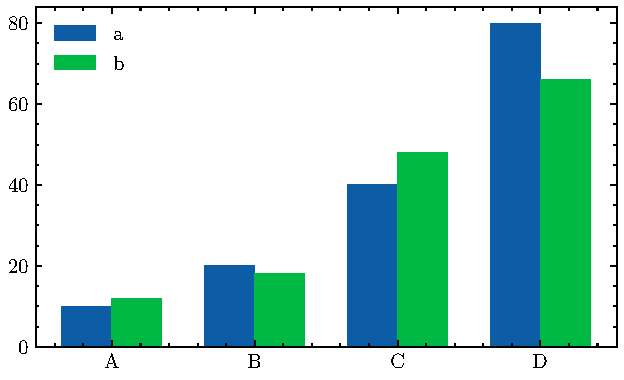
\includegraphics[width=0.9\textwidth]{fig-bar.pdf}
\end{center}
}

\codebox{Histogram}{
\color{codeFont}
\texttt{> fig, ax = plt.subplots(figsize=(5,3)) \\
> ax.hist(data3, bins=20, density=True,  \\
. \ \ \ \ \ \ \ histtype='step', label='a') \\
> ax.hist(data4, bins=20, density=True,  \\
. \ \ \ \ \ \ \ histtype='step', label='b') \\
> ax.legend()\vspace{-0.15cm}
}
\color{mainFont}
\begin{center}
	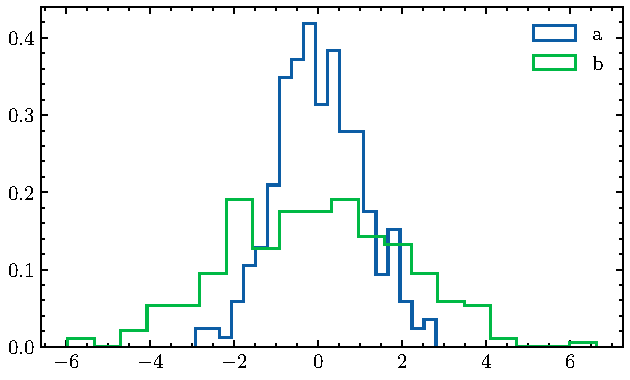
\includegraphics[width=0.9\textwidth]{fig-hist.pdf}
\end{center}\vspace{-0.15cm}
\texttt{density=True}: area under histogram $=1$.
}

\codebox{Pie Chart}{
\color{codeFont}
\texttt{> fig, ax = plt.subplots(figsize=(4,4))\\
> ax.pie(data1, \\
. \ \ \ \ \ \ explode=[0, 0, .08, 0], \\
. \ \ \ \ \ \ labels=labels, \\
. \ \ \ \ \ \ autopct='\%1.1f\textbackslash\%\%', \\
. \ \ \ \ \ \ startangle = 90, \\
. \ \ \ \ \ \ counterclock = False)\\
> ax.axis('equal')
}
\color{mainFont}
\begin{center}
	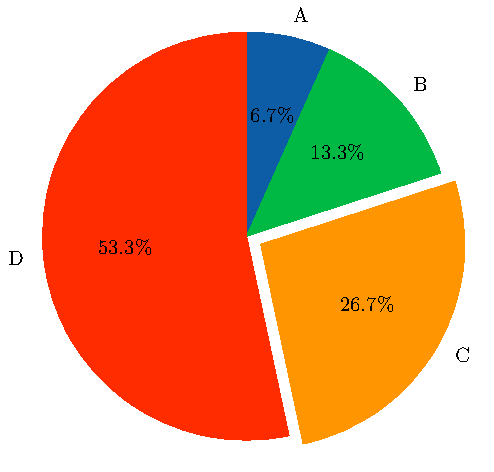
\includegraphics[width=0.5\textwidth]{fig-pie-chart.pdf}
\end{center}
}

\codebox{Contour Plot}{
\color{codeFont}
\texttt{> fig, ax = plt.subplots(figsize=(5,3)) \\
> c = ax.contour(X, Y, Z, levels=6) \\
> ax.clabel(c, inline=True, fmt='\%1.1f')
}\vspace{-0.3cm}
\color{mainFont}
\begin{center}
	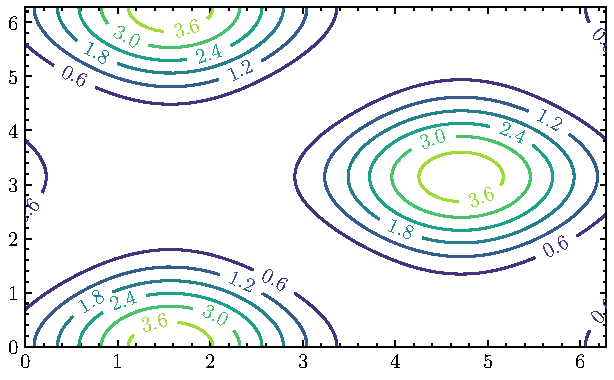
\includegraphics[width=0.9\textwidth]{fig-contour.pdf}
\end{center}
}

\codebox{Filled Contour Plot}{
\color{codeFont}
\texttt{> fig, ax = plt.subplots(figsize=(5,3)) \\
> c = ax.contourf(X, Y, Z, levels=6) \\
> cbar = fig.colorbar(c) \\
> cbar.ax.set\_ylabel('value') 
}
\color{mainFont}
\begin{center}
	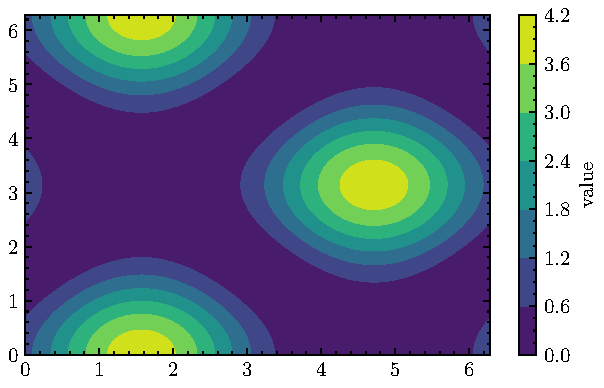
\includegraphics[width=0.9\textwidth]{fig-contourf.pdf}
\end{center}
}

\codebox{3D Parametric Plot}{
\color{codeFont}
\texttt{> fig, ax = plt.subplots(figsize=(3,3), \\
. \ subplot\_kw=\{"projection":\ "3d"\}) \\
> ax.plot(np.cos(4*t), np.sin(4*t), t)\\
> plt.savefig('a.pdf', transparent=True)\\[-14pt]
}
\color{mainFont}
\begin{center}
	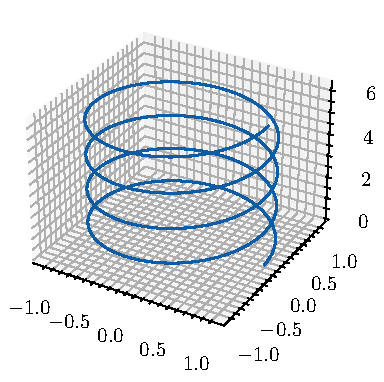
\includegraphics[width=0.7\textwidth]{fig-3d-parametric.pdf}
\end{center}
}

\codebox{3D Surface Plot}{
\color{codeFont}
\texttt{> from matplotlib import cm \\
> fig, axes = plt.subplots(1, 2, \\
. \ \ \ \ \ subplot\_kw=\{"projection":\ "3d"\}, \\
. \ \ \ \ \ figsize=(8,4))\\
> ax = axes[0] \\
> ax.plot\_surface(X, Y, Z, \\
. \ \ \ \ \ \ \ \ \ \ \ \ \ \ \ cmap=cm.coolwarm) \\
> ax = axes[1] \\
> ax.plot\_surface(X, Y, Z, alpha=0.3) \\
> ax.contour(X, Y, Z, zdir='x', \\
. \ \ \ \ \ \ \ \ \ \ offset=X.min(), \\
. \ \ \ \ \ \ \ \ \ \ cmap=cm.coolwarm) \\
> ax.contour(X, Y, Z, zdir='y', \\
. \ \ \ \ \ \ \ \ \ \ offset=Y.max(), \\
. \ \ \ \ \ \ \ \ \ \ cmap=cm.coolwarm) \\
> ax.contour(X, Y, Z, zdir='z', \\
. \ \ \ \ \ \ \ \ \ \ offset=Z.min(), \\
. \ \ \ \ \ \ \ \ \ \ cmap=cm.coolwarm) 
}
\color{mainFont}
\begin{center}
	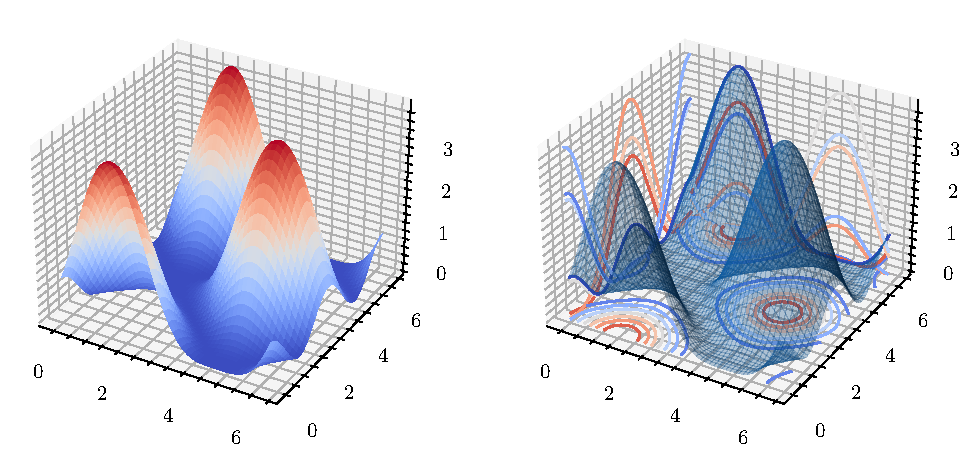
\includegraphics[width=\textwidth]{fig-3d-surface.pdf}
\end{center}
}

\end{multicols}


\end{document}







